\documentclass[border=7pt]{standalone}
\usepackage{tikz}
\begin{document}
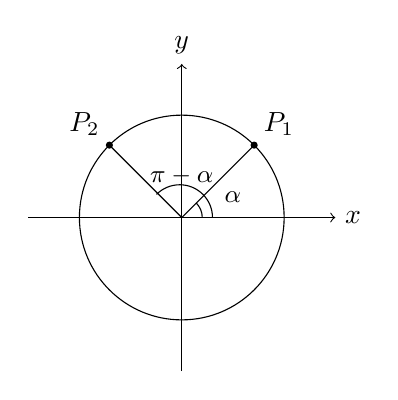
\begin{tikzpicture}[scale=1.3]
   \draw (0,0) circle (1cm);
   \draw[->] (-1.5,0) -- (1.5,0)node[anchor=west]{$x$};
   \draw[->] (0,-1.5) -- (0,1.5) node[anchor=south] {$y$};
   %P_1
   \draw (0.2,0) arc(0:45:0.2);
   \draw  (0.5,0.2) node{\small$\alpha$};
   \draw (0,0)--(45:1) node[anchor=south west]{$P_1$}; %(-0.707106781,0.707106781-4)
   \fill (45:1) circle(1pt);
   %P_2
   \draw (0,0)--(135:1)node[anchor=south east]{$P_2$};%(0.707106781,0.707106781-4) ;
   \draw (0.3,0) arc(0:135:0.32);
   \draw (0,0.4) node{\small $\pi - \alpha$};
   \fill (135:1) circle(1pt);
\end{tikzpicture}
\end{document}
